\documentclass[11pt]{article}

\usepackage[a4paper,margin=2.6cm,headheight=14pt]{geometry}
\usepackage[T1]{fontenc}
\usepackage[utf8]{inputenc}
\usepackage[sc]{mathpazo}          % Palatino: text + math
\linespread{1.06}
\usepackage{microtype}
\usepackage{amsmath}
\usepackage{graphicx}
\usepackage{booktabs}
\usepackage{float}
\usepackage{caption}
\usepackage{enumitem}
\usepackage{setspace}
\usepackage{xcolor}
\usepackage{titlesec}
\usepackage{fancyhdr}

\definecolor{accent}{HTML}{064A56}
\definecolor{ink}{HTML}{1E2A2C}
\definecolor{muted}{HTML}{6B7A7D}

\color{ink}

\titleformat{\section}{\Large\bfseries\color{accent}}{\thesection}{0.8em}{}
\titleformat{\subsection}{\large\bfseries\color{accent}}{\thesubsection}{0.7em}{}
\titlespacing{\section}{0pt}{1.6em}{0.7em}
\titlespacing{\subsection}{0pt}{1.1em}{0.45em}

\captionsetup{font={small},labelfont={bf,color=accent},skip=6pt}
\setlist{itemsep=2pt,topsep=4pt,parsep=0pt}

\pagestyle{fancy}
\fancyhf{}
\fancyhead[L]{\small\color{muted} Freight Rate Prediction}
\fancyhead[R]{\small\color{muted} Machine Learning Engineer Assessment}
\fancyfoot[C]{\small\color{muted} \thepage}
\renewcommand{\headrulewidth}{0.4pt}
\renewcommand{\headrule}{\color{accent!40}\hrule width\headwidth height 0.4pt}

\newcommand{\code}[1]{\texttt{#1}}

\begin{document}

% ------------------------------------------------------------- title
\begin{center}
    {\color{accent}\rule{\textwidth}{1.6pt}}\\[14pt]
    {\LARGE\bfseries\color{accent} Freight Rate Prediction}\\[6pt]
    {\large Machine Learning Engineer Assessment --- Technical Report}\\[10pt]
    {\small\color{muted} LightGBM regression on 48{,}000 labeled truckload loads
    \quad$\cdot$\quad October 2025 holdout MAPE: 4.63\,\%}\\[10pt]
    {\color{accent}\rule{\textwidth}{1.6pt}}
\end{center}

\vspace{4pt}
\begin{center}
\begin{minipage}{0.92\textwidth}
\small
\textbf{\color{accent}Summary.}\quad
This report describes a regression model that predicts the posted rate of
truckload freight loads. The model is a gradient-boosted tree ensemble
(LightGBM) trained on the logarithm of the posted rate with an
$L_1$ objective. It was developed on 48{,}000 loads from January--October
2025 and validated on a strict time-based holdout: training on
January--September, testing on October, the month immediately preceding the
November--December prediction window. On that holdout the model achieves a
mean absolute error of \$117.77 (4.63\,\% MAPE, 2.71\,\% median APE,
$R^2 = 0.837$). The final model is refit on all ten months as a five-seed
ensemble and used to score the 12{,}000 validation loads and the fixed
December reference-lane chart.
\end{minipage}
\end{center}

% ------------------------------------------------------------- 1
\section{Task and Data}

The task is to predict the posted rate---the dollar amount a load was posted
for---of 12{,}000 truckload loads dated November 1 to December 31, 2025.
Table~\ref{tab:datasets} summarizes the three input files. Each load is
described by its pickup and delivery city with coordinates, distance,
equipment type, weight, date, and two market signals
(\code{market\_index}, \code{quote\_signal}). The training file additionally
contains the target, \code{posted\_rate}.

\begin{table}[H]
\centering\small
\caption{Datasets used in this project.}
\label{tab:datasets}
\begin{tabular}{@{}llll@{}}
\toprule
\textbf{File} & \textbf{Rows} & \textbf{Period} & \textbf{Role} \\
\midrule
\code{train\_test.csv}       & 48{,}000 & Jan--Oct 2025 & labeled development data \\
\code{validation.csv}        & 12{,}000 & Nov--Dec 2025 & final scoring (no labels) \\
\code{december\_chart\_inputs.csv} & 31 & Dec 2025 & fixed-lane daily rate chart \\
\bottomrule
\end{tabular}
\end{table}

% ------------------------------------------------------------- 2
\section{What the Data Shows}

Three findings shaped every later decision.

\textbf{Pricing is multiplicative and distance-led.} Distance alone
correlates with the posted rate at 0.91, and the relationship is close to a
power law: a model as simple as $\textit{rate} = 5.12 \times
\textit{distance}^{0.87}$ already explains most of the variance
(Figure~\ref{fig:distance}). Rate per mile declines with distance---long
hauls price lower per mile---and is roughly log-normally distributed around a
median of \$2.15/mi. This is why the model predicts $\log(\textit{rate})$
rather than the raw dollar amount.

\begin{figure}[H]
\centering
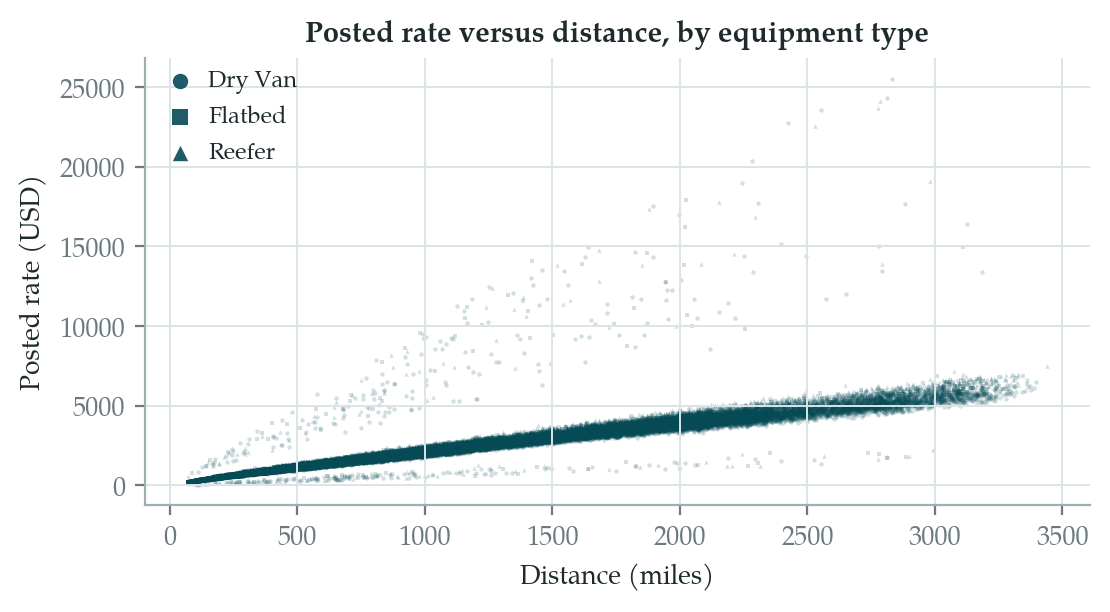
\includegraphics[width=0.98\textwidth]{report_assets/rate_vs_distance.png}
\caption{Posted rate versus distance for the three equipment types
(marker shapes). The tight multiplicative band around the distance trend is
the dominant structure in the data.}
\label{fig:distance}
\end{figure}

\textbf{The market index carries the time signal.} Mean daily rate per mile
correlates 0.58 with \code{market\_index}, and the monthly pattern tracks it
closely (Figure~\ref{fig:monthly}). At daily granularity the market index
shows a weekly sawtooth---rates climb through the week and dip on
weekends---which later reappears in the December forecast. Equipment mix also
matters: Reefer loads price about 13\,\% above Dry Van per mile, Flatbed
about 8\,\%. Heavier loads price slightly higher per mile.
\code{quote\_signal} adds only a weak incremental signal (row-level
correlation $\approx 0.06$).

\begin{figure}[H]
\centering
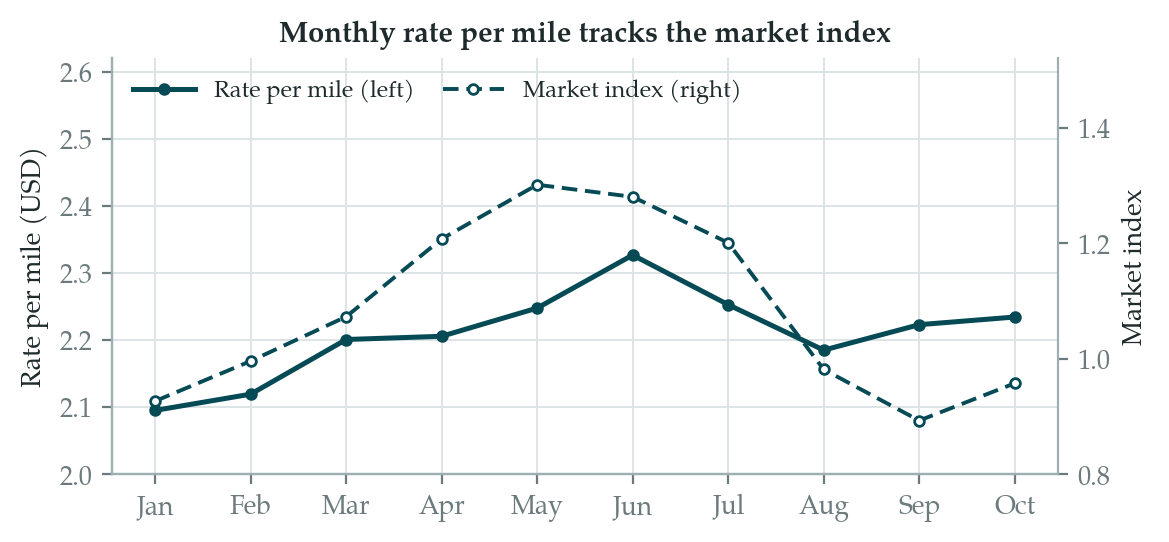
\includegraphics[width=0.98\textwidth]{report_assets/monthly_trend.png}
\caption{Monthly mean rate per mile (solid) against the monthly mean market
index (dashed). The two series move together, so the model can rely on
\code{market\_index}---which is provided for the scoring period---instead of
calendar features that would not generalize to unseen months.}
\label{fig:monthly}
\end{figure}

\textbf{The scoring period reaches beyond the training map.} The validation
set introduces eight cities that never appear in training (e.g.\ Chicago,
Charlotte, San Diego) and 1{,}461 loads on previously unseen
origin--destination pairs. A model that memorizes lanes cannot handle this;
one that reasons from geography, distance, and market conditions can.

% ------------------------------------------------------------- 3
\section{Data Quality}

The data is clean overall. Three issues required explicit handling:

\begin{itemize}
\item \textbf{Implausible rates.} 152 training rows (0.3\,\%) have a
rate per mile below \$0.50 or above \$10.00---values outside any plausible
truckload market range and consistent with data-entry or unit errors (one
load is posted at \$25{,}533). These rows were removed from training
(Figure~\ref{fig:rpm}); the $L_1$ training objective provides further
robustness to any that remain.
\item \textbf{Missing values.} \code{weight} is missing for 300 rows and
\code{market\_index} for 374 (about 0.7\,\% each), spread evenly across
months and equipment types---consistent with missingness at random. LightGBM
handles missing values natively, so no imputation was applied and the
scoring data (which has the same pattern) is treated identically.
\item \textbf{Identifiers.} \code{load\_id} values are unique within each
file and disjoint across files, so there is no leakage through identifiers.
City coordinates are constant per city and identical across files, making
them a reliable geographic encoding.
\end{itemize}

\begin{figure}[H]
\centering
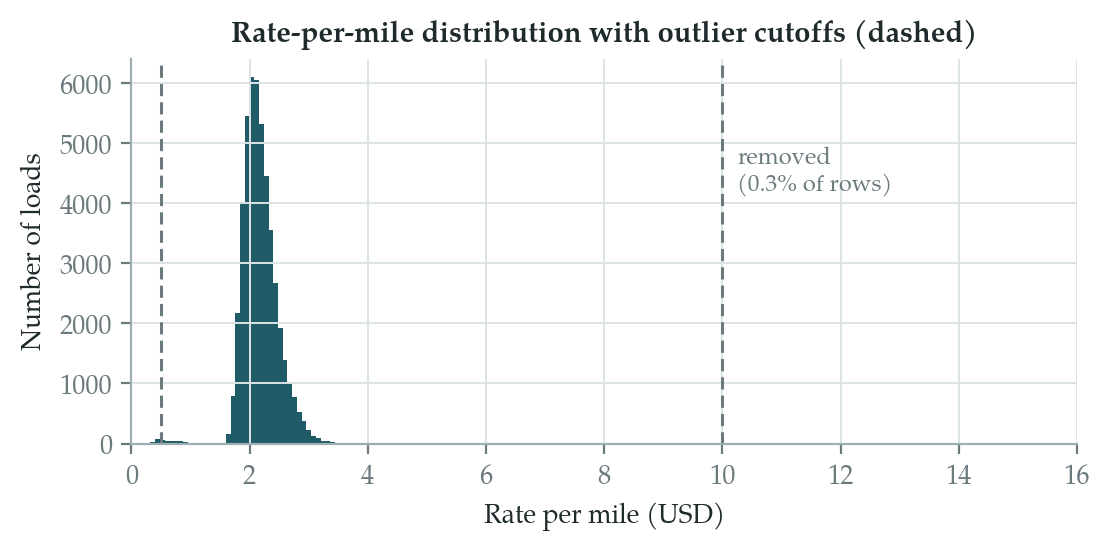
\includegraphics[width=0.98\textwidth]{report_assets/rpm_distribution.png}
\caption{Rate-per-mile distribution of the training data. Rows outside the
dashed cutoffs (\$0.50--\$10.00 per mile) were excluded from training.}
\label{fig:rpm}
\end{figure}

% ------------------------------------------------------------- 4
\section{Validation Strategy}

The central design choice is to validate \emph{in time}, not at random.
The development data was split at a calendar boundary: the model trains on
January--September and is tested on October---the month immediately before
the November--December scoring window. This mirrors the real task, in which
the future must be predicted from the past.

A random split would make reported accuracy look better than it is. Loads
from the same lane and the same market week appear throughout the year, so
randomly scattered test rows would leak lane-level and market-level patterns
across the boundary. The October holdout avoids this and doubles as a
rehearsal for the true scoring conditions.

All model selection---objective, target transform, feature set, tree
size---was performed against this holdout only. After selection, the final
model was refit on all ten months (47{,}848 cleaned rows) using the
early-stopped iteration count, with five seeds trained and averaged in log
space to reduce variance.

% ------------------------------------------------------------- 5
\section{Model}

The model is a LightGBM gradient-boosted tree ensemble trained on
$\log(\texttt{posted\_rate})$ with an $L_1$ objective. Gradient boosting
suits this problem for four reasons: the relationships are non-linear and
rich in interactions (lane $\times$ equipment $\times$ market); the data is
tabular and mid-sized; native categorical support handles the 64 cities
without fragile one-hot encoding; and missing values are handled natively.
The log transform matches the multiplicative error structure, and the $L_1$
objective is robust to the heavy right tail of posted rates.

Table~\ref{tab:features} lists the features. Two candidate features were
tested and deliberately excluded. The raw route string
($\sim$4{,}000 origin--destination pairs) slightly overfit relative to city
and coordinate features, and a calendar-month feature cannot generalize to
November and December---months never seen in training; its place is taken by
\code{market\_index} and day-of-week, which are available at scoring time.

\begin{table}[H]
\centering\small
\caption{Model features. Distances, coordinates and market signals are used
as-is; cities, equipment and day-of-week are native categoricals.}
\label{tab:features}
\begin{tabular}{@{}ll@{}}
\toprule
\textbf{Group} & \textbf{Features} \\
\midrule
Lane geometry   & \code{distance}, \code{log(distance)}, pickup/delivery latitude \& longitude \\
Categoricals    & \code{equipment}, \code{pickup}, \code{delivery}, day-of-week \\
Load            & \code{weight} \\
Market          & \code{market\_index}, \code{quote\_signal} \\
\bottomrule
\end{tabular}
\end{table}

Table~\ref{tab:comparison} shows the configuration comparison on the October
holdout. The shipped configuration achieves the lowest error; every
alternative was rejected empirically.

\begin{table}[H]
\centering\small
\caption{Model configuration comparison on the October holdout
(single seed). The first row is the shipped configuration.}
\label{tab:comparison}
\begin{tabular}{@{}lcc@{}}
\toprule
\textbf{Configuration} & \textbf{MAE (\$)} & \textbf{MAPE} \\
\midrule
\textbf{$L_1$ on $\log(\text{rate})$, shipped feature set} & \textbf{115.16} & \textbf{4.54\,\%} \\
\quad + raw route string as categorical   & 115.69 & 4.57\,\% \\
\quad raw target instead of $\log(\text{rate})$ & 115.59 & 4.62\,\% \\
\quad without coordinates                 & 118.58 & 4.71\,\% \\
\quad without day-of-week                 & 115.30 & 4.63\,\% \\
\quad $L_2$ objective instead of $L_1$    & 124.58 & 4.76\,\% \\
\quad Tweedie objective                   & 125.60 & 4.89\,\% \\
\quad + calendar month (leakage-risk probe) & 121.23 & 4.62\,\% \\
\bottomrule
\end{tabular}
\end{table}

% ------------------------------------------------------------- 6
\section{Results}

On the October holdout (4{,}831 loads) the model achieves the metrics in
Table~\ref{tab:metrics}. Half of all predictions land within 2.71\,\% of the
actual rate. RMSE is considerably larger than MAE because a handful of
extreme loads---legitimate but rare---dominate squared error; the median and
MAPE are the more representative figures for typical loads.

\begin{table}[H]
\centering\small
\caption{October 2025 holdout metrics (train: January--September).}
\label{tab:metrics}
\begin{tabular}{@{}lr@{}}
\toprule
\textbf{Metric} & \textbf{Value} \\
\midrule
Mean absolute error (MAE)        & \$117.77 \\
Median absolute percentage error & 2.71\,\% \\
Mean absolute percentage error   & 4.63\,\% \\
Root mean squared error          & \$612.74 \\
$R^2$                            & 0.837 \\
\bottomrule
\end{tabular}
\end{table}

Figure~\ref{fig:pva} shows predicted versus actual rates on the holdout:
predictions track the diagonal tightly across the full price range, with no
systematic bias for cheap or expensive loads. Feature importance
(Figure~\ref{fig:importance}) confirms the exploratory analysis---distance
dominates, followed by the two market signals and weight, with geography and
equipment contributing the remainder.

\begin{figure}[H]
\centering
\begin{minipage}{0.48\textwidth}
    \centering
    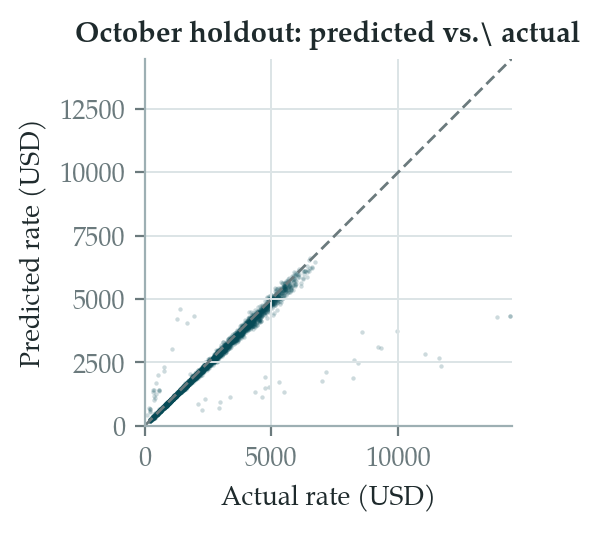
\includegraphics[width=\textwidth]{report_assets/predicted_vs_actual.png}
    \caption{Predicted versus actual rates on the October holdout.}
    \label{fig:pva}
\end{minipage}\hfill
\begin{minipage}{0.48\textwidth}
    \centering
    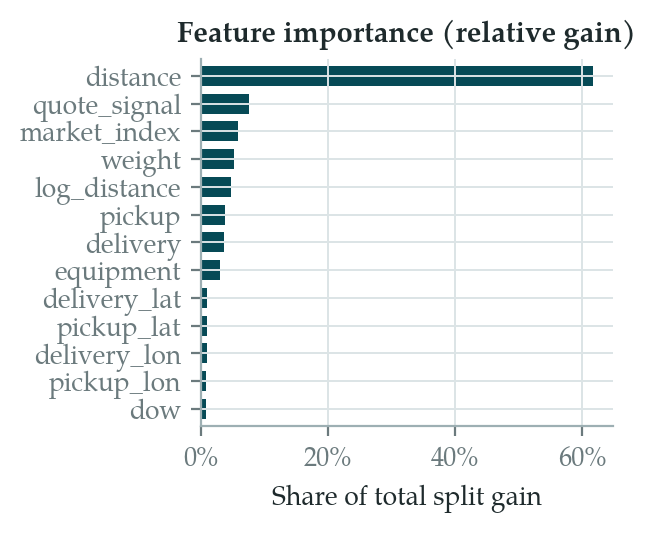
\includegraphics[width=\textwidth]{report_assets/feature_importance.png}
    \caption{Feature importance as share of total split gain.}
    \label{fig:importance}
\end{minipage}
\end{figure}

% ------------------------------------------------------------- 7
\section{December Reference-Lane Forecast}

The December chart fixes every attribute of a load---Lexington to Fort Wayne,
360 miles, Dry Van, 32{,}000 lb---and varies only the date. Its inputs,
however, carry no market signals or coordinates. Coordinates were attached
from the city lookup; \code{market\_index} and \code{quote\_signal} were
estimated per December date from the daily means observed in the
validation data, which covers December 2025 (with the last 30 training days
as fallback).

The resulting curve (Figure~\ref{fig:december}) reproduces the weekly
sawtooth of the market index and peaks in Christmas week, ranging from
\$791 to \$820. This is consistent with the lane's history: the 32 training
loads on this lane averaged \$857 at a higher average market level than
December's.

\begin{figure}[H]
\centering
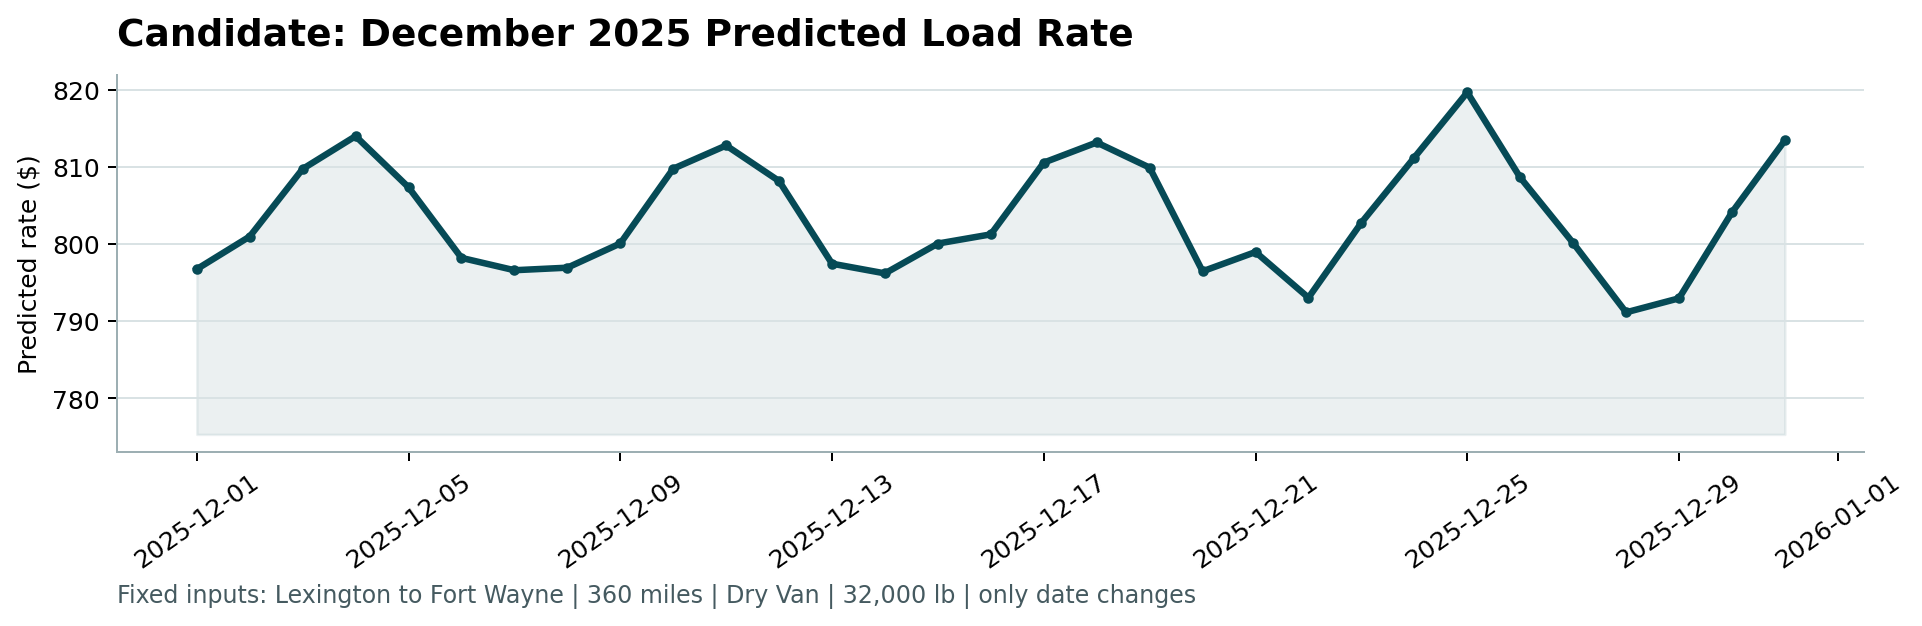
\includegraphics[width=0.98\textwidth]{scorer_results/candidate_december.png}
\caption{Fixed December 2025 prediction chart produced by \code{score.py}
from the model's daily predictions for the reference lane.}
\label{fig:december}
\end{figure}

% ------------------------------------------------------------- 8
\section{Reproducibility}

The full pipeline regenerates every artifact---models, figures, predictions,
chart, and this report---with fixed seeds and byte-identical outputs:

\begin{center}
\begin{minipage}{0.9\textwidth}
\begin{small}
\begin{verbatim}
python -m pip install -r requirements.txt
python src/train.py        # holdout metrics, figures, final models
python src/predict.py      # validation_predictions.csv + December inputs
python src/make_figures.py # EDA figures
python score.py --predictions validation_predictions.csv \
    --december-predictions data/december_chart_inputs.csv
\end{verbatim}
\end{small}
\end{minipage}
\end{center}

\noindent The scorer validates both output files (12{,}000 predictions and 31
December rows) and regenerates Figure~\ref{fig:december}.

% ------------------------------------------------------------- 9
\section{Conclusion}

\begin{sloppypar}
A deliberately simple, leakage-free pipeline---time-based validation, a
log-target $L_1$ gradient-boosting model, and features chosen to generalize
to unseen cities and months---predicts truckload spot rates to within
about 4.6\,\% on a holdout that faithfully rehearses the scoring task. The
same pipeline produces the required 12{,}000 predictions and the fixed
December rate chart, and every number in this report can be regenerated with
three commands.
\end{sloppypar}

\end{document}
